\documentclass{beamer}

\pdfmapfile{+sansmathaccent.map}


\mode<presentation>
{
	\usetheme{Warsaw} % or try Darmstadt, Madrid, Warsaw, Rochester, CambridgeUS, ...
	\usecolortheme{seahorse} % or try seahorse, beaver, crane, wolverine, ...
	\usefonttheme{serif}  % or try serif, structurebold, ...
	\setbeamertemplate{navigation symbols}{}
	\setbeamertemplate{caption}[numbered]
} 


%%%%%%%%%%%%%%%%%%%%%%%%%%%%
% itemize settings


%%%%%%%%%%%%%%%%%%%%%%%%%%%%
% itemize settings

\definecolor{myhotpink}{RGB}{255, 80, 200}
\definecolor{mywarmpink}{RGB}{255, 60, 160}
\definecolor{mylightpink}{RGB}{255, 80, 200}
\definecolor{mypink}{RGB}{255, 30, 80}
\definecolor{mydarkpink}{RGB}{155, 25, 60}

\definecolor{mypaleblue}{RGB}{240, 240, 255}
\definecolor{mylightblue}{RGB}{120, 150, 255}
\definecolor{myblue}{RGB}{90, 90, 255}
\definecolor{mygblue}{RGB}{70, 110, 240}
\definecolor{mydarkblue}{RGB}{0, 0, 180}
\definecolor{myblackblue}{RGB}{40, 40, 120}

\definecolor{myblackturquoise}{RGB}{5, 53, 60}
\definecolor{mydarkdarkturquoise}{RGB}{8, 93, 110}
\definecolor{mydarkturquoise}{RGB}{28, 143, 150}
\definecolor{mypaleturquoise}{RGB}{230, 255, 255}
\definecolor{myturquoise}{RGB}{48, 213, 200}

\definecolor{mygreen}{RGB}{0, 200, 0}
\definecolor{mydarkgreen}{RGB}{0, 120, 0}
\definecolor{mygreen2}{RGB}{245, 255, 230}

\definecolor{mygrey}{RGB}{120, 120, 120}
\definecolor{mypalegrey}{RGB}{160, 160, 160}
\definecolor{mydarkgrey}{RGB}{80, 80, 160}

\definecolor{mydarkred}{RGB}{160, 30, 30}
\definecolor{mylightred}{RGB}{255, 150, 150}
\definecolor{myred}{RGB}{200, 110, 110}
\definecolor{myblackred}{RGB}{120, 40, 40}


\definecolor{myblackmaroon}{RGB}{50, 0, 15}

\definecolor{mygreen}{RGB}{0, 200, 0}
\definecolor{mygreen2}{RGB}{205, 255, 200}

\definecolor{mydarkcolor}{RGB}{60, 25, 155}
\definecolor{mylightcolor}{RGB}{130, 180, 250}

\setbeamertemplate{itemize items}[default]

\setbeamertemplate{itemize item}{\color{myblackmaroon}$\blacksquare$}
\setbeamertemplate{itemize subitem}{\color{mydarkdarkturquoise}$\blacktriangleright$}
\setbeamertemplate{itemize subsubitem}{\color{mygray}$\blacksquare$}

\setbeamercolor{palette quaternary}{fg=white,bg=myblackmaroon}
\setbeamercolor{titlelike}{parent=palette quaternary}

\setbeamercolor{palette quaternary2}{fg=black,bg=mypaleblue}
\setbeamercolor{frametitle}{parent=palette quaternary2}

\setbeamerfont{frametitle}{size=\Large,series=\scshape}
\setbeamerfont{framesubtitle}{size=\normalsize,series=\upshape}





%%%%%%%%%%%%%%%%%%%%%%%%%%%%
% block settings

\setbeamercolor{block title}{bg=red!30,fg=black}

\setbeamercolor*{block title example}{bg=mygreen!40!white,fg=black}

\setbeamercolor*{block body example}{fg= black, bg= mygreen2}


%%%%%%%%%%%%%%%%%%%%%%%%%%%%
% URL settings
\hypersetup{
	colorlinks=true,
	linkcolor=blue,
	filecolor=blue,      
	urlcolor=blue,
}

%%%%%%%%%%%%%%%%%%%%%%%%%%

\renewcommand{\familydefault}{\rmdefault}

\usepackage{amsmath}
\usepackage{mathtools}

\usepackage{subcaption}

\usepackage{qrcode}

\DeclareMathOperator*{\argmin}{arg\,min}
\newcommand{\bo}[1] {\mathbf{#1}}

\newcommand{\R}{\mathbb{R}} 
\newcommand{\T}{^\top}     



\newcommand{\mydate}{Fall 2023}

\newcommand{\mygit}{\textcolor{blue}{\href{https://github.com/SergeiSa/Mechatronics-2023}{github.com/SergeiSa/Mechatronics-2023}}}

\newcommand{\myqr}{ \textcolor{black}{\qrcode[height=1.5in]{https://github.com/SergeiSa/Mechatronics-2023}}
}

\newcommand{\myqrframe}{
	\begin{frame}
		\centerline{Lecture slides are available via Github, links are on Moodle}
		\bigskip
		\centerline{You can help improve these slides at:}
		\centerline{\mygit}
		\bigskip
		\myqr
	\end{frame}
}


\newcommand{\bref}[2] {\textcolor{blue}{\href{#1}{#2}}}

%%%%%%%%%%%%%%%%%%%%%%%%%%%%
% code settings

\usepackage{listings}
\usepackage{color}
% \definecolor{mygreen}{rgb}{0,0.6,0}
% \definecolor{mygray}{rgb}{0.5,0.5,0.5}
\definecolor{mymauve}{rgb}{0.58,0,0.82}
\lstset{ 
	backgroundcolor=\color{white},   % choose the background color; you must add \usepackage{color} or \usepackage{xcolor}; should come as last argument
	basicstyle=\footnotesize,        % the size of the fonts that are used for the code
	breakatwhitespace=false,         % sets if automatic breaks should only happen at whitespace
	breaklines=true,                 % sets automatic line breaking
	captionpos=b,                    % sets the caption-position to bottom
	commentstyle=\color{mygreen},    % comment style
	deletekeywords={...},            % if you want to delete keywords from the given language
	escapeinside={\%*}{*)},          % if you want to add LaTeX within your code
	extendedchars=true,              % lets you use non-ASCII characters; for 8-bits encodings only, does not work with UTF-8
	firstnumber=0000,                % start line enumeration with line 0000
	frame=single,	                   % adds a frame around the code
	keepspaces=true,                 % keeps spaces in text, useful for keeping indentation of code (possibly needs columns=flexible)
	keywordstyle=\color{blue},       % keyword style
	language=Octave,                 % the language of the code
	morekeywords={*,...},            % if you want to add more keywords to the set
	numbers=left,                    % where to put the line-numbers; possible values are (none, left, right)
	numbersep=5pt,                   % how far the line-numbers are from the code
	numberstyle=\tiny\color{mygray}, % the style that is used for the line-numbers
	rulecolor=\color{black},         % if not set, the frame-color may be changed on line-breaks within not-black text (e.g. comments (green here))
	showspaces=false,                % show spaces everywhere adding particular underscores; it overrides 'showstringspaces'
	showstringspaces=false,          % underline spaces within strings only
	showtabs=false,                  % show tabs within strings adding particular underscores
	stepnumber=2,                    % the step between two line-numbers. If it's 1, each line will be numbered
	stringstyle=\color{mymauve},     % string literal style
	tabsize=2,	                   % sets default tabsize to 2 spaces
	title=\lstname                   % show the filename of files included with \lstinputlisting; also try caption instead of title
}


%%%%%%%%%%%%%%%%%%%%%%%%%%%%
% URL settings
\hypersetup{
	colorlinks=false,
	linkcolor=blue,
	filecolor=blue,      
	urlcolor=blue,
}

%%%%%%%%%%%%%%%%%%%%%%%%%%

%%%%%%%%%%%%%%%%%%%%%%%%%%%%
% tikz settings

\usepackage{tikz}
\tikzset{every picture/.style={line width=0.75pt}}


\title{Gaits}
\subtitle{Contact-aware Control, Lecture 10}
\author{by Sergei Savin}
\centering
\date{\mydate}



\begin{document}
\maketitle


\begin{frame}{Content}

\begin{itemize}
\item Bipedal walking
\item Inverted pendulum - model
\item Inverted pendulum walking
\item Inverted pendulum - illustration
\item Spring-Loaded Inverted Pendulum
\item Raibert-style footstep planning
\end{itemize}

\end{frame}




\begin{frame}{Bipedal walking, 1}
	% \framesubtitle{Parameter estimation}
	\begin{flushleft}
		
		Bipedal walking and running can be broken into phases:
		
		\begin{itemize}
			\item \emph{double-support} - two feet touch the ground;
			
			\item \emph{single-support} - one foot touches the ground;
			
			\item \emph{flight phase} - no foot touches the ground.
		\end{itemize}
		
		\bigskip
		
		 Running is defined as gate that includes a flight phase; walking doesn't.
		
		\bigskip
		
		Simple model of walking includes single-support phase only (when one foot touches the ground, the other leaves it at the same time).
		
	\end{flushleft}
\end{frame}



\begin{frame}{Bipedal walking, 2}
	% \framesubtitle{Parameter estimation}
	\begin{flushleft}
		
		A single-support phase walking is characterized by step length, time allocated for a single step, velocity of the center of mass, position of the next support (place where the foot lands). These values are not independent.
		
		\bigskip
		
		Double-support walking is additionally characterized by the duration of the double-support phase.
		
		\bigskip
		
		We can identify two popular approaches to generating gates:
		
		\begin{itemize}
			\item Raibert-style approach: we decide on the desired center of mass velocity and compute step length (position of the next foothold).
			
			\item ZMP-style approach: we decide sequence of footholds and compute the center of mass trajectory.
		\end{itemize}
		
		
	\end{flushleft}
\end{frame}




\begin{frame}{Inverted pendulum - model}
	% \framesubtitle{Parameter estimation}
	\begin{flushleft}
		
		Let us consider an inverted pendulum:
		
		\begin{equation}
			J \ddot \varphi + lmg \cos(\varphi) = 0.
		\end{equation}
		
		Kinetic energy $T$ and potential energy $P$ of the system are defined as:
		
		\begin{align}
			T = \frac{J \dot \varphi^2}{2}, \ \ \ \ P =  \cos(\varphi) lmg.
		\end{align}
		
		Assuming no dissipation of energy and no actuation, the total energy of the system is conserved:
		
		\begin{align}
			\frac{J \dot \varphi^2}{2} + \cos(\varphi) lmg = \text{const}
		\end{align}
		
		
		
	\end{flushleft}
\end{frame}




\begin{frame}{Inverted pendulum walking, 1}
	% \framesubtitle{Parameter estimation}
	\begin{flushleft}
		
		Let us model a single support walking phase as inverted pendulum moving from the time $t_1$ when the angle $\varphi(t_1) = \alpha$ to the time $t_2$ when the angle $\varphi(t_2) = \beta$.
		
		\bigskip
		
		Potential energy at the beginning of the single-support phase the potential energy $P_1 = \cos(\alpha) lmg$ and angular velocity $\omega_1 = \dot \varphi(t_1)$, and the end of the single-support phase it is $P_2 = \cos(\beta) lmg$ and $\omega_2 = \dot \varphi(t_2)$.
		
		\bigskip
		
		Total energy is conserved:
		
		\begin{align}
			\frac{J \omega_1^2}{2} + \cos(\alpha) lmg = 
			\frac{J \omega_2^2}{2} + \cos(\beta) lmg
			\\
			\cos(\beta)  - \cos(\alpha)= 
			\frac{J }{2lmg} (\omega_1^2 - \omega_2^2)
		\end{align}
		
	\end{flushleft}
\end{frame}



\begin{frame}{Inverted pendulum walking, 2}
	% \framesubtitle{Parameter estimation}
	\begin{flushleft}
		
		Thus we have the following relation between $\omega_1$ and $\omega_2$:
		%
		\begin{align}
			\omega_1^2 - \omega_2^2
			=
			\frac{2lmg}{J}
			(\cos(\beta)  - \cos(\alpha))
		\end{align}
	%
	where $|\alpha| < \frac{\pi}{2}$ and $|\beta| < \frac{\pi}{2}$.
	
		\bigskip
	
		If $|\beta| = |\alpha|$, the r.h.s. of the equation becomes 0, hence $\omega_1 = \omega_2$.
		
		\bigskip
		
		If $|\beta| > |\alpha|$, the r.h.s. of the equation is negative, hence $\omega_1 < \omega_2$.
		
		\bigskip
		
		If $|\beta| < |\alpha|$, the r.h.s. of the equation is positive, hence $\omega_1 > \omega_2$.

		
	\end{flushleft}
\end{frame}



\begin{frame}{Inverted pendulum - illustration 1}
	
	
	
	\tikzset{every picture/.style={line width=0.75pt}} %set default line width to 0.75pt        
	
	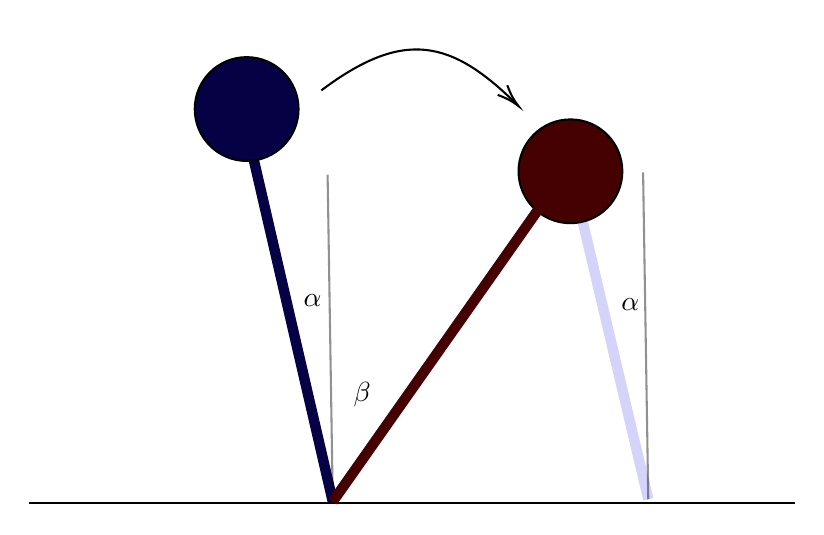
\begin{tikzpicture}[x=0.75pt,y=0.75pt,yscale=-1,xscale=1]
		%uncomment if require: \path (0,300); %set diagram left start at 0, and has height of 300
		
		%Straight Lines [id:da6833931113886613] 
		\draw    (46,299.6) -- (415,299.6) ;
		%Straight Lines [id:da7426943888769713] 
		\draw [color={rgb, 255:red, 6; green, 0; blue, 69 }  ,draw opacity=1 ][line width=3.75]    (152.5,126.1) -- (165.97,184.37) -- (192.5,299.1) ;
		%Shape: Circle [id:dp34607384744867664] 
		\draw  [fill={rgb, 255:red, 6; green, 0; blue, 69 }  ,fill opacity=1 ] (126,110) .. controls (126,96.19) and (137.19,85) .. (151,85) .. controls (164.81,85) and (176,96.19) .. (176,110) .. controls (176,123.81) and (164.81,135) .. (151,135) .. controls (137.19,135) and (126,123.81) .. (126,110) -- cycle ;
		%Straight Lines [id:da7866042378074112] 
		\draw [color={rgb, 255:red, 0; green, 0; blue, 0 }  ,draw opacity=0.43 ]   (190,141.6) -- (192.5,299.1) ;
		%Shape: Circle [id:dp17880604409163348] 
		\draw  [fill={rgb, 255:red, 69; green, 0; blue, 2 }  ,fill opacity=1 ] (282,140) .. controls (282,126.19) and (293.19,115) .. (307,115) .. controls (320.81,115) and (332,126.19) .. (332,140) .. controls (332,153.81) and (320.81,165) .. (307,165) .. controls (293.19,165) and (282,153.81) .. (282,140) -- cycle ;
		%Straight Lines [id:da4764217442897467] 
		\draw [color={rgb, 255:red, 69; green, 0; blue, 2 }  ,draw opacity=1 ][line width=3.75]    (297,150.6) -- (192.5,299.1) ;
		%Straight Lines [id:da006148065593531982] 
		\draw [color={rgb, 255:red, 90; green, 87; blue, 239 }  ,draw opacity=0.26 ][line width=3.75]    (313,164.6) -- (344.5,298) ;
		%Straight Lines [id:da9623807221368184] 
		\draw [color={rgb, 255:red, 0; green, 0; blue, 0 }  ,draw opacity=0.43 ]   (342,140.5) -- (344.5,298) ;
		%Curve Lines [id:da7492478712462101] 
		\draw    (187,101) .. controls (226.6,71.3) and (249.54,76.49) .. (281.04,107.65) ;
		\draw [shift={(282,108.6)}, rotate = 225] [color={rgb, 255:red, 0; green, 0; blue, 0 }  ][line width=0.75]    (10.93,-3.29) .. controls (6.95,-1.4) and (3.31,-0.3) .. (0,0) .. controls (3.31,0.3) and (6.95,1.4) .. (10.93,3.29)   ;
		
		% Text Node
		\draw (177,198) node [anchor=north west][inner sep=0.75pt]   [align=left] {$\displaystyle \alpha $};
		% Text Node
		\draw (201,240) node [anchor=north west][inner sep=0.75pt]   [align=left] {$\displaystyle \beta $};
		% Text Node
		\draw (330,200) node [anchor=north west][inner sep=0.75pt]   [align=left] {$\displaystyle \alpha $};
		
		
	\end{tikzpicture}
\end{frame}


%%%%%%%%%%%%%%%%%%%%%%%%%%%%%%%%%%%%%

\begin{frame}{Inverted pendulum walking, 3}
	% \framesubtitle{Parameter estimation}
	\begin{flushleft}
		
		The pendulum model indicates that, if we want to increase kinetic energy, we need to decrease the angle $|\alpha|$ by absolute value. If we fix $\beta$, this corresponds to a shorter step length.
		
		\bigskip
		
		If we want to decrease the kinetic energy, we need to increase the angle $|\alpha|$ by absolute value. If we fix $\beta$ and $\alpha < 0$ (the pendulum is in the II quadrant at the beginning of the support phase), this corresponds to a longer step length.
		
	\end{flushleft}
\end{frame}


\begin{frame}{Inverted pendulum walking - illustration 2}
	
	
	\tikzset{every picture/.style={line width=0.75pt}} %set default line width to 0.75pt        
	
	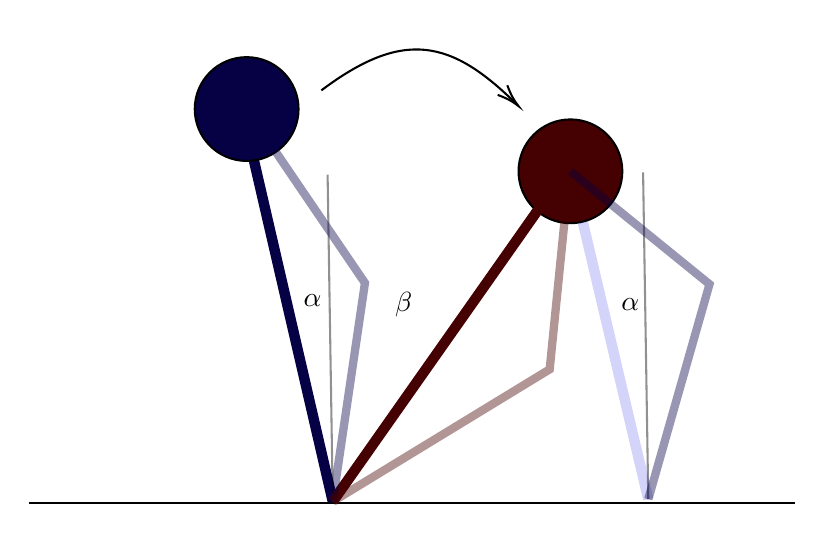
\begin{tikzpicture}[x=0.75pt,y=0.75pt,yscale=-1,xscale=1]
		%uncomment if require: \path (0,300); %set diagram left start at 0, and has height of 300
		
		%Straight Lines [id:da9054839042619105] 
		\draw    (46,299.6) -- (415,299.6) ;
		%Straight Lines [id:da03903544935564618] 
		\draw [color={rgb, 255:red, 6; green, 0; blue, 69 }  ,draw opacity=1 ][line width=3.75]    (152.5,126.1) -- (165.97,184.37) -- (192.5,299.1) ;
		%Shape: Circle [id:dp49096758082222247] 
		\draw  [fill={rgb, 255:red, 6; green, 0; blue, 69 }  ,fill opacity=1 ] (126,110) .. controls (126,96.19) and (137.19,85) .. (151,85) .. controls (164.81,85) and (176,96.19) .. (176,110) .. controls (176,123.81) and (164.81,135) .. (151,135) .. controls (137.19,135) and (126,123.81) .. (126,110) -- cycle ;
		%Straight Lines [id:da7152856305819504] 
		\draw [color={rgb, 255:red, 0; green, 0; blue, 0 }  ,draw opacity=0.43 ]   (190,141.6) -- (192.5,299.1) ;
		%Shape: Circle [id:dp9292224828625106] 
		\draw  [fill={rgb, 255:red, 69; green, 0; blue, 2 }  ,fill opacity=1 ] (282,140) .. controls (282,126.19) and (293.19,115) .. (307,115) .. controls (320.81,115) and (332,126.19) .. (332,140) .. controls (332,153.81) and (320.81,165) .. (307,165) .. controls (293.19,165) and (282,153.81) .. (282,140) -- cycle ;
		%Straight Lines [id:da337630158558913] 
		\draw [color={rgb, 255:red, 69; green, 0; blue, 2 }  ,draw opacity=1 ][line width=3.75]    (297,150.6) -- (192.5,299.1) ;
		%Straight Lines [id:da6854535438885112] 
		\draw [color={rgb, 255:red, 90; green, 87; blue, 239 }  ,draw opacity=0.26 ][line width=3.75]    (313,164.6) -- (344.5,298) ;
		%Straight Lines [id:da10179232205063693] 
		\draw [color={rgb, 255:red, 0; green, 0; blue, 0 }  ,draw opacity=0.43 ]   (342,140.5) -- (344.5,298) ;
		%Curve Lines [id:da8665568123690086] 
		\draw    (187,101) .. controls (226.6,71.3) and (249.54,76.49) .. (281.04,107.65) ;
		\draw [shift={(282,108.6)}, rotate = 225] [color={rgb, 255:red, 0; green, 0; blue, 0 }  ][line width=0.75]    (10.93,-3.29) .. controls (6.95,-1.4) and (3.31,-0.3) .. (0,0) .. controls (3.31,0.3) and (6.95,1.4) .. (10.93,3.29)   ;
		%Straight Lines [id:da7719465406872958] 
		\draw [color={rgb, 255:red, 6; green, 0; blue, 69 }  ,draw opacity=0.41 ][line width=3]    (151,110) -- (208,193.8) -- (192.5,299.1) ;
		%Straight Lines [id:da7377496644189505] 
		\draw [color={rgb, 255:red, 69; green, 0; blue, 1 }  ,draw opacity=0.41 ][line width=3]    (306,145.4) -- (297,235.4) -- (192.5,299.1) ;
		%Straight Lines [id:da921787689217114] 
		\draw [color={rgb, 255:red, 6; green, 0; blue, 69 }  ,draw opacity=0.41 ][line width=3]    (307,140) -- (374,194.4) -- (344.5,298) ;
		
		% Text Node
		\draw (177,198) node [anchor=north west][inner sep=0.75pt]   [align=left] {$\displaystyle \alpha $};
		% Text Node
		\draw (221,197) node [anchor=north west][inner sep=0.75pt]   [align=left] {$\displaystyle \beta $};
		% Text Node
		\draw (330,200) node [anchor=north west][inner sep=0.75pt]   [align=left] {$\displaystyle \alpha $};
		
		
	\end{tikzpicture}
	
	
\end{frame}



\begin{frame}{Human running}
	% \framesubtitle{Parameter estimation}
	\begin{flushleft}
		
		This model visually corresponds to how humans run:
		
		% TODO: \usepackage{graphicx} required
		\begin{figure}
			\centering
			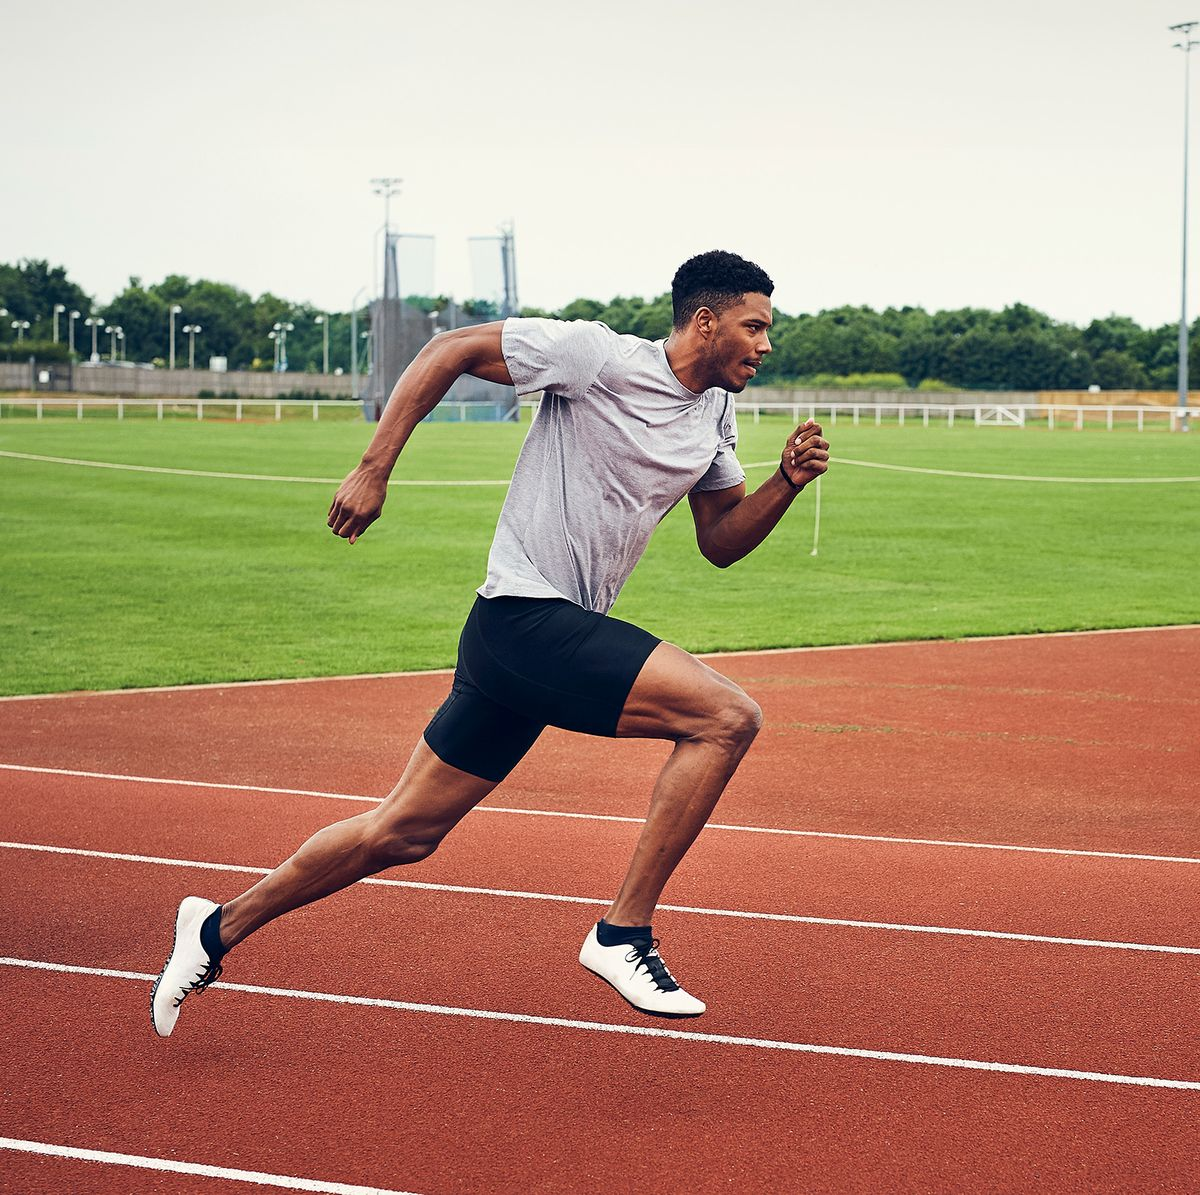
\includegraphics[width=0.5\linewidth]{running-track}
			\caption{ \bref{https://www.runnersworld.com/uk/training/beginners/a33455616/running-track/}{Credit: runnersworld.com} }
			\label{fig:running-track}
		\end{figure}
		
		
	\end{flushleft}
\end{frame}




\begin{frame}{Spring-Loaded Inverted Pendulum (SLIP), 1}
	% \framesubtitle{Parameter estimation}
	\begin{flushleft}
		
		Since the total energy of the system of the pendulum remains, if the kinetic energy of the end of the single-support phase increased, it means the potential energy decreased by the same value. It implies that the center of mass lowered its position at the end of the single-support phase compared with its start. Given a constant $\alpha$, it would imply a "shorter leg" during the next single-support phase.
		
		
		\bigskip
		
		We can solve this problem by introducing a loaded spring into the robot leg. The deformation of the spring is related to the change of the leg length. Stiffness of the spring is a hyper-parameter.
		
		\bigskip
		
		 This idea is quite natural: during walking with positive acceleration, people step on a leg partially bent at the knee (effective length between the foot at the hip is lower) which then rapidly straightens.
		
	\end{flushleft}
\end{frame}




\begin{frame}{Spring-Loaded Inverted Pendulum (SLIP), 2}
	% \framesubtitle{Parameter estimation}
	\begin{flushleft}
		
		By introducing a flight phase, we solve the problem of spring "pulling" on the mass.
		
		\bigskip
		
		% TODO: \usepackage{graphicx} required
		\begin{figure}
			\centering
			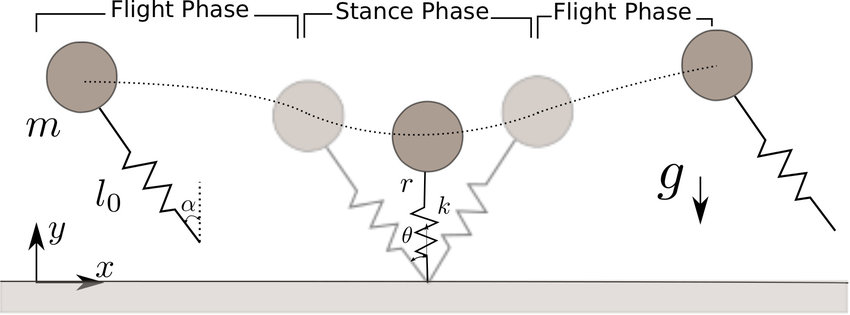
\includegraphics[width=0.9\linewidth]{Spring-Loaded-Inverted-Pendulum}
			\caption{Credit: Dai, H. and Tedrake, R., 2012. Optimizing robust limit cycles for legged locomotion on unknown terrain}
			\label{fig:spring-loaded-inverted-pendulum}
		\end{figure}
		
		
		
	\end{flushleft}
\end{frame}




\begin{frame}{Raibert-style footstep planning, 1}
	% \framesubtitle{Parameter estimation}
	\begin{flushleft}
		
		Assuming forward motion (no change in orientation), we can propose the following formula for computing the next step location:
		
		\begin{equation}
			p_k = r_\text{CoM} +  r_s + v \Delta t + k (v - v_\text{des})
		\end{equation}
		%
		where $p_k$ the next step position, $r_\text{CoM}$ - center of mass (CoM) position, $r_s$ - vector from CoM to the robot shoulder,  $\Delta t$ - step time, $v$ - CoM velocity, $v_\text{des}$ - desired CoM velocity and $k$ - gain coefficient.
		
		
	\end{flushleft}
\end{frame}


\begin{frame}{Raibert-style footstep planning, 2}
	% \framesubtitle{Parameter estimation}
	\begin{flushleft}
		
		\begin{itemize}
			\item If $v_\text{des} > v$, the component $ k (v - v_\text{des})$ is negative, hence the step becomes \textbf{shorter}.
			
			\item If $v_\text{des} < v$, the component $ k (v - v_\text{des})$ is positive, hence the step becomes \textbf{longer}.
			
			\item If $v_\text{des} = v$, the component $ k (v - v_\text{des})$ is equal to zero, hence the step remains the same.
		\end{itemize}
	
		\bigskip
		
		This corresponds to what we had earlier: fixing $\beta$ shorter step corresponds to a smaller $\alpha$, hence more kinetic energy at the end of the single-support phase, and vice-versa.
		
	\end{flushleft}
\end{frame}





\begin{frame}{Read more}
	\begin{itemize}
		\item M. H. Raibert, H. B. Brown, and M. Chepponis, “Experiments in Balance with a 3D One-Legged Hopping Machine,” The International Journal of Robotics Research, vol. 3, no. 2, pp. 75–92, 1984.
		
	\end{itemize}
\end{frame}



\myqrframe

\end{document}
